\section{Współczynnik modyfikujący średnią rozkładu}

Dodatkowy współczynnik modyfikujący średnią rozkładu został dodany do funkcji aktualizującej opinię danego agenta.
Okazało się, że współczynnik wynoszący 500 jest odpowiedni dla uzyskania więcej niż jednej zbieżnej grupy, przynajmniej dla sieci Watts-Strogatz [\ref{fig:Watts-Strogatz_plot_example}] i Barabási-Albert [\ref{fig:Barabási-Albert_plot_example}].
W przypadku sieci Erdős-Rényi [\ref{fig:Erdos-Renyi_plot_example}] nie powstaje więcej niż jedna grupa,
raczej pojawiają się "orbitujące" elementy populacji, znacznie oddalone od głównej grupy.
Dla mniejszych współczynników populacja jest zbieżna do jednej grupy, a dla większych elementy przestają się grupować.
Przykładowe rezultaty widoczne są poniżej.

\begin{figure}
    \centering
    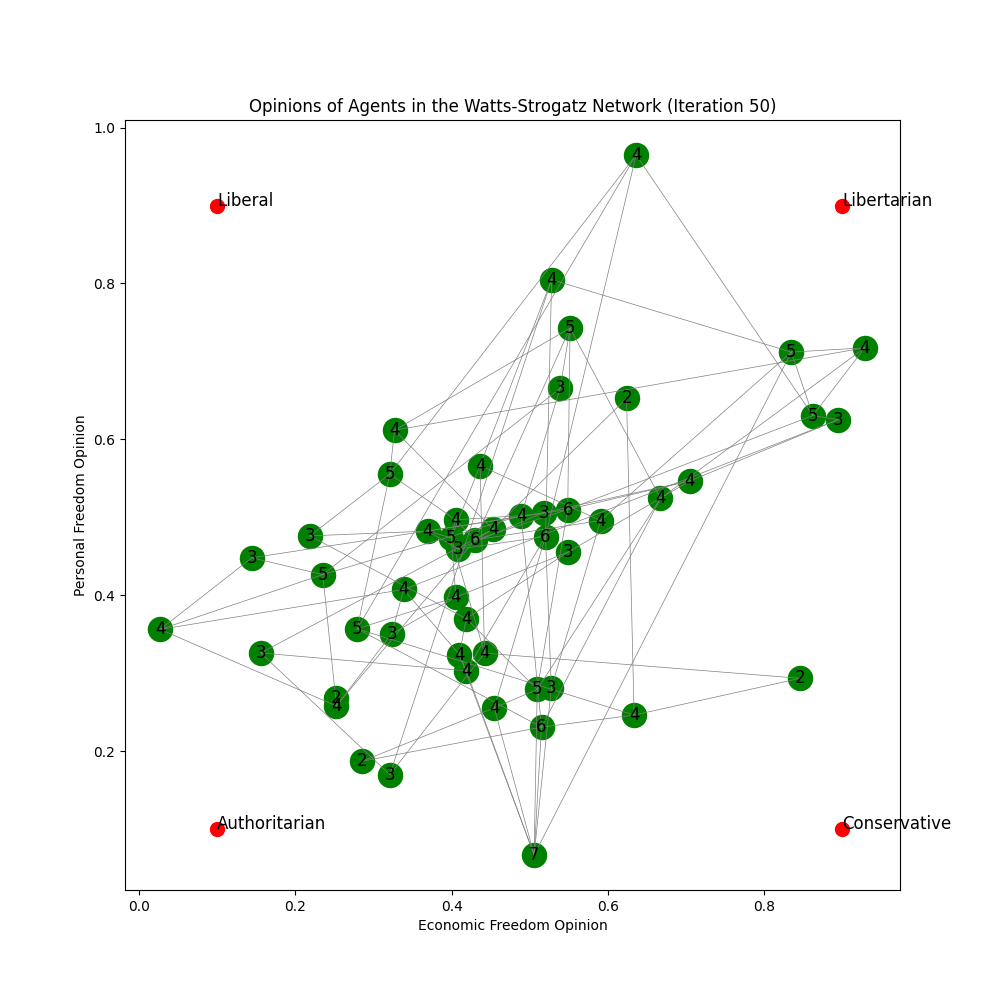
\includegraphics[width=0.5\textwidth]{img/Watts-Strogatz.png}
    \caption{Sieć Watts-Strogatz w iteracji nr 50}
    \label{fig:Watts-Strogatz_plot_example}
\end{figure}

\begin{figure}
    \centering
    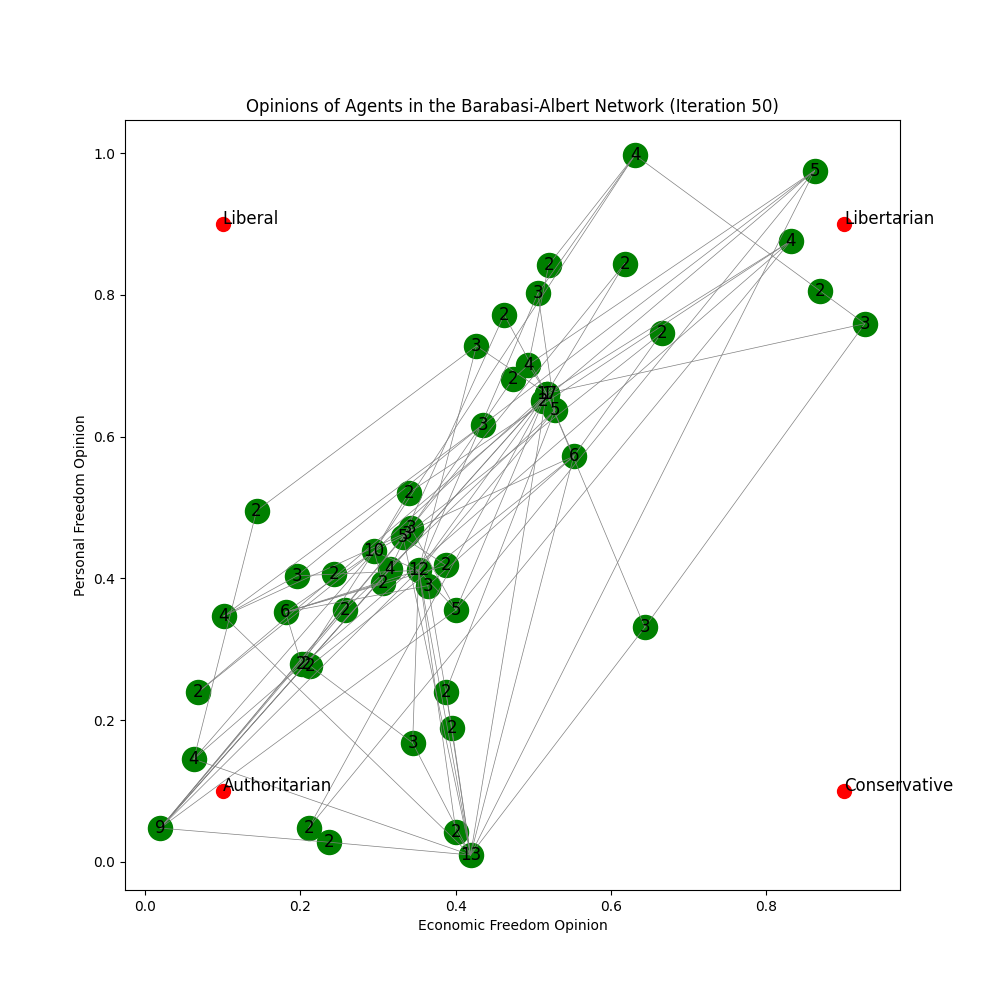
\includegraphics[width=0.5\textwidth]{img/Barabasi-Albert.png}
    \caption{Sieć Barabási-Albert w iteracji nr 50}
    \label{fig:Barabási-Albert_plot_example}
\end{figure}

\begin{figure}
    \centering
    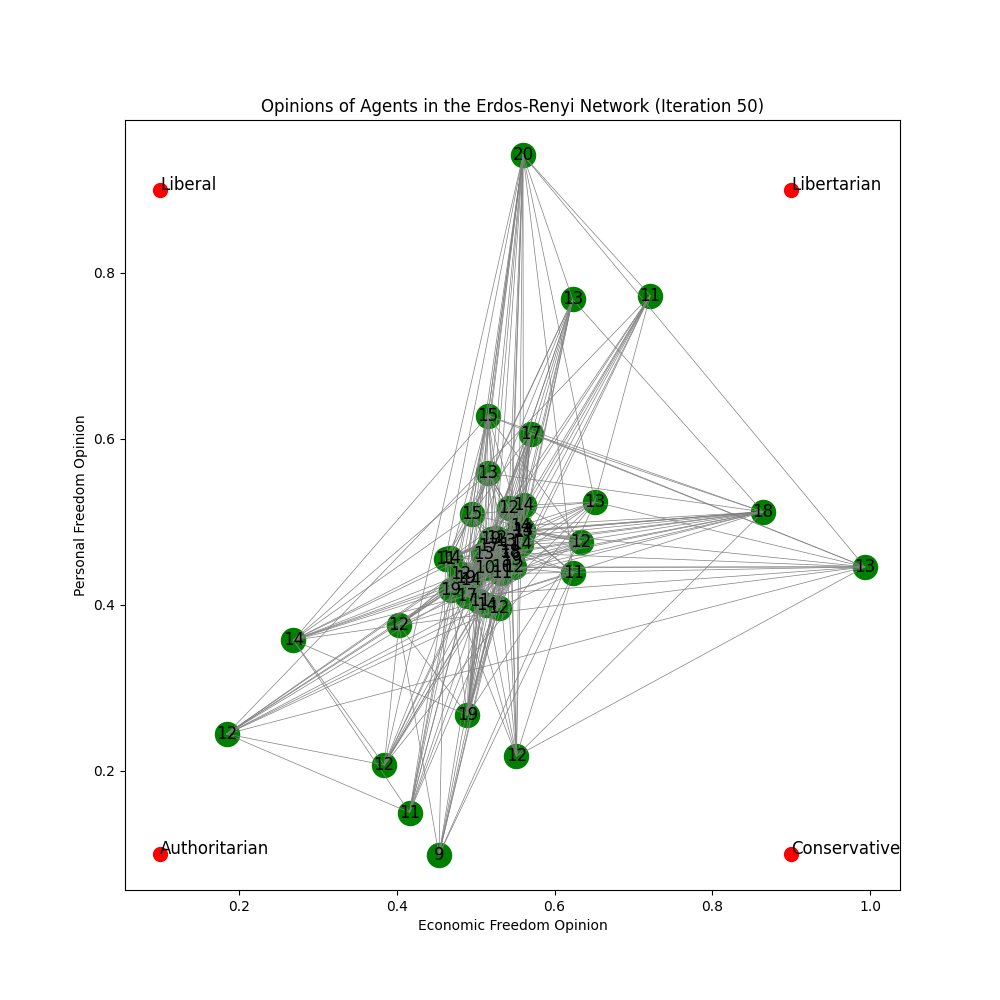
\includegraphics[width=0.5\textwidth]{img/Erdos-Renyi.png}
    \caption{Sieć Erdős-Rényi w iteracji nr 50}
    \label{fig:Erdos-Renyi_plot_example}
\end{figure}
